\chapter{Analisis Persoalan dan Rancangan Solusi}
\label{chapter:analisis-persoalan-dan-rancangan-solusi}

Tujuan utama penulisan bab ini adalah untuk menjelaskan proses solusi atas masalah pencarian kondisi ketika \textit{erasure coding} memiliki \textit{response time} yang lebih cepat dibandingkan replikasi. Bagian ini memaparkan proses analisis masalah, rancangan solusi, serta implementasi solusi.


\section{Analisis}

\section{Analisis Permasalahan}
\label{sec:analisis-permasalahan}

% Berdasarkan latar belakang yang telah diuraikan pada \ref{sec:latar-belakang}, penggunaan \textit{erasure coding} pada sebuah sistem dapat mengurangi kebutuhan penyimpanan data dengan tetap menjaga integritas dan ketahanan data. Walaupun membutuhkan sumber daya komputasi dalam penerapannya, pengurangan ukuran data keseluruhan yang diperlukan menyebabkan juga turunnya ukuran data yang perlu dikirim ke \textit{node} lainnya.Hal ini menyebabkan mungkinnya terdapat suatu kondisi ketika {response time} yang diperlukan untuk melakukan operasi pada \textit{erasure coding} lebih rendah jika dibandingkan dengan melakukan operasi yang sama pada sistem yang menggunakan \textit{replikasi} untuk mencapai ketahanan tersebut.

Berdasarkan latar belakang dan studi literatur yang telah ditentukan, \textit{erasure coding} memiliki potensi untuk menghasilkan \textit{response time} yang lebih rendah dibandingkan dengan sistem berbasis \textit{replikasi} karena walaupun membutuhkan komputasi, ukuran data yang dikirimkan untuk ketahanan lebih rendah dibandingkan replikasi. Riset ini akan menganalisis faktor-faktor untuk mencapai kondisi tersebut. Faktor yang dianalisis antara lain ukuran data yang besar dan jaringan yang lambat. Dengan demikian, diperlukan sistem yang dapat mensimulasikan operasi pada sistem \textit{erasure coding} dan replikasi sekaligus memvariasikan faktor-faktor tersebut dalam operasinya tanpa memengaruhi kinerja sistem di sisi lain.

Dari permasalahan tersebut, dirumuskan kebutuhan sebuah perangkat lunak antara lain
\begin{enumerate}

    \item Sistem harus dapat mensimulasikan kondisi \textit{database} terdistribusi yang menggunakan replikasi ataupun \textit{erasure coding}.
    \item Sistem harus dapat menyimpan data secara \textit{persistent}.
    \item Sistem harus dapat memvariasikan ukuran data dan kecepatan jaringan.
    \item Sistem harus dapat menjalankan eksperimen berulang kali untuk mendapatkan data dari eksperimen.

\end{enumerate}

Penjelasan lebih detail mengenai kebutuhan sistem terdapat pada lampiran \ref{sec:rancangan-struktural}.

\subsection{Alternatif Solusi}
\label{sec:alternatif-solusi}

Berdasarkan permasalahan pada bagian \ref{sec:analisis-permasalahan}, terdapat berbagai macam alternatif solusi untuk menyelesaikan permasalahan tersebut. Pada penelitian ini, solusi yang dipilih adalah dengan membuat sistem yang mengkombinasikan Memcached sebagai \textit{in-memory key value store} dengan RocksDB sebagai \textit{persistent storage} dengan Reed-Solomon sebagai algoritma \textit{erasure coding}.

\subsubsection{Perbandingan Pengembangan Sistem}

Terdapat beberapa solusi yang dipertimbangkan dalam pembangunan sistem, yaitu membangun sistem dengan 

\begin{enumerate}
  \item Mengembangkan sistem secara modular dengan in-memory key-value store dan persistent storage terpisah
  
  Pendekatan ini mengkombinasikan antara sistem \textit{in-memory key-value store} dengan menggunakan \textit{database} terpisah sebagai tempat penyimpanan data \textit{persistence}. Replikasi dan \textit{erasure coding} dapat dilakukan pada data persisten yang disimpan pada \textit{database} tersebut. Kelebihan dari pendekatan ini adalah kemudahan dari implementasi dibandingkan pengembangan sendiri ataupun modifikasi \textit{database} yang sudah lebih kompleks. Namun, kekurangannya adalah \textit{overhead} penggunaan memori dari menjalankan \textit{in-memory key-value store} dan \textit{database} terpisah. Dari ketiga alternatif solusi, kemudahan implementasi dan kekurangan yang dapat ditoleransi menjadikan alternatif ini solusi yang dipilih dalam penelitian ini.


  \item Mengembangkan sistem mock database
  
  Pendekatan ini membangun semua fitur-fitur yang dibutuhkan secara mandiri. Kelebihan dari pendekatan ini kebebasan yang tinggi sehingga sistem dapat disesuaikan untuk eksperimen. Namun, pendekatan ini sulit mencerminkan kondisi nyata. Selain itu, kinerja sistem yang dikembangkan juga bergantung erat pada waktu serta kemampuan pengembangan peneliti.

  \item Mengembangkan sistem yang sudah memiliki fitur in memory database dan persistent storage
  
  Pengembangan ini membangun mengganti fitur yang dibutuhkan untuk penelitian di atas \textit{database} lebih kompleks dari Memcached. Pendekatan ini memiliki kelebihan kedekatan kondisi eksperimen dengan dunia nyata. Namun, pendekatan ini sulit dilakukan karena membutuhkan waktu yang lama untuk memahami dan mengubah \textit{source-code database} yang kompleks.
\end{enumerate}

\subsubsection{Perbandingan Kakas}
Setelah menentukan solusi pengembangan sistem secara modular, terdapat beberapa kakas yang dapat dipilih untuk solusi tersebut. Disebabkan pemilihan solusi modular, kakas yang dipertimbangkan untuk digunakan meliputi kakas \textit{in-memory key-value store} dan kakas untuk \textit{persistent database}.

\begin{enumerate}
    \item In-memory key-value store
    
    Memcached dipilih sebagai \textit{in-memory key-value store}. Selain Memcached, kakas yang dipertimbangkan untuk digunakan sebagai \textit{in-memory key-value store} adalah seperti yang ada pada tabel \ref{tab:tools-kv} \parencite{redis_docs} \parencite{dragonflydb_docs} \parencite{memcached_docs}.

    \begin{table}[h]
        \centering
        \caption{Perbandingan kakas in-memory key-value store}
        \resizebox{\textwidth}{!}{
            \begin{tabular}{|l|p{5cm}|p{5cm}|p{3cm}|}
                \hline
                \rowcolor{black!10} Kakas & Kelebihan & Kekurangan & Notes \\ \hline
                Redis & +Support struktur data kompleks \newline +Support transaksi kompleks & -Single Threaded \newline -Kompleks & Ada support untuk replikasi \\ \hline
                DragonflyDB & +Multithreaded \newline +Support struktur data kompleks \newline +Support transaksi kompleks & -Lebih kompleks dari Memcached, lebih simpel dari Redis \newline -Relatif baru, komunitas terbatas dibanding kedua alternatif & Rilis 2023, Ada support untuk replikasi\\ \hline
                Memcached & +Simpel \newline +Multithreaded & -Struktur data terbatas \newline -Transaksi terbatas & Sangat minimalis \\ \hline
            \end{tabular}
        }
        \label{tab:tools-kv}
    \end{table}

    Dari kakas-kakas tersebut, dipilih Memcached sebagai kakas untuk eksperimen ini. Alasan utama pemilihan Memcached adalah sifatnya yang paling simpel, kinerja \textit{multithreaded}-nya, serta tidak dibutuhkannya fitur-fitur yang dimiliki Redis dan Dragonfly.
    
    \item Persistent database
    
    RocksDB dipilih sebagai \textit{persistent storage} karena berfokus pada kinerja \textit{write} yang tinggi. Penggunaan RocksDB juga dilakukan seperti \textit{library} sehingga memudahkan pengembangan sistem yang modular. Selain RocksDB, kakas yang dipertimbangkan untuk digunakan sebagai \textit{persistent database} adalah seperti yang ada pada tabel \ref{tab:tools-db} \parencite{cassandra_docs} \parencite{scylladb_docs} \parencite{rocksdb_docs} \parencite{leveldb_docs} \parencite{mongodb_docs}.

    \begin{table}[h]
        \centering
        \caption{Perbandingan kakas persistent database}
        \resizebox{\textwidth}{!}{
            \begin{tabular}{|l|p{5cm}|p{5cm}|p{3cm}|}
                \hline
                \rowcolor{black!10} Kakas & Kelebihan & Kekurangan & Notes \\ \hline
                Cassandra & +Horizontal Scalability baik \newline +Sudah ada referensi implementasi erasure coding pada paper lain & -Eventual Consistency \newline -Latensi tinggi untuk operasi write \newline -Sangat Kompleks & Utamanya Wide-Column Store\\ \hline
                ScyllaDB & +Lebih efisien dan performant dibandingkan Cassandra \newline +Memiliki pilihan strong consistency & -Lebih kompleks dibandingkan Cassandra \newline -Ekosistem terbatas & Mirip dan kompatibel dengan Cassandra. \\ \hline
                RocksDB & +Kinerja tinggi untuk operasi write \newline +Recovery menggunakan write ahead log & -Single Node \newline -Keterbatasan pada concurrent writes & Pengembangan LevelDB\\ \hline
                LevelDB & +Simpel \newline +Penggunaan memori kecil \newline +Kinerja tinggi untuk operasi write & -Fitur terbatas seperti compression dan data terbatas pada string \newline -Operasi write skala besar masih lebih lambat dibandingkan RocksDB \newline -Keterbatasan pada concurrent writes & Dasar dari RocksDB\\ \hline
                MongoDB & +Support query kompleks \newline +Penggunaan fleksibel & -Operasi kurang optimal \newline -Konsumsi memori besar \newline -Storage overhead besar & Utamanya Dokumen database\\ \hline
            \end{tabular}
        }
        \label{tab:tools-db}
    \end{table}

    Dari kakas-kakas tersebut, dipilih RocksDB sebagai kakas untuk eksperimen ini. Selain RocksDB, LevelDB juga merupakan kandidat yang kuat untuk eksperimen ini karena sifatnya yang simpel. Namun, pada akhirnya, RocksDB dipilih karena pengembangannya yang masih aktif, kinerja \textit{write} yang lebih tinggi, serta fitur-fitur tambahan seperti \textit{compression} dan penyimpanan data dalam \textit{byte}.

\end{enumerate}

\subsubsection{Perbandingan Algoritma Erasure Coding}
Terdapat beberapa algoritma yang dipertimbangkan untuk implementasi \textit{erasure coding} selain Reed-Solomon \parencite{manasse2009reed}. Algoritma tersebut antara lain adalah kode LDPC (\textit{Low-Density Parity-Check}) \parencite{gallagher1962ldpc}, kode BCH (\textit{Bose-Chaudhuri-Hocquenghem}) \parencite{bose1960bch}, algoritma berbasis XOR (Terdapat berbagai macam sumber dan implementasi untuk algoritma XOR), kode Fountain \parencite{asteris2014fountain}, dan \textit{Regenerating Codes} \parencite{rashmi2012regenerating}. Berikut perbandingan masing-masing algoritma 

\begin{table}[ht]
    \centering
    \caption{Perbandingan algoritma erasure coding}
    \resizebox{\textwidth}{!}{
        \begin{tabular}{|l|l|p{3cm}|p{2.2cm}|p{3cm}|p{3cm}|}
            \hline
            \rowcolor{black!10} Algoritma & Basis & Komputasi & Distance & Kelebihan & Kekurangan \\ \hline
            Reed-Solomon & Block level & Polynomial Interpolation & Optimal & Efisiensi penyimpanan tinggi & Komputasi kompleks \\ \hline
            LDPC Codes & Bit level & Sparse Matrix operations & Hampir \newline Optimal & Kecepatan \textit{encoding/decoding} tinggi untuk \textit{data streaming} & Membutuhkan \textit{overhead} untuk operasi \textit{block}  \\ \hline
            BCH Codes & Block level & Syndrome decoding & Optimal & Efisien untuk \textit{burst errors} & Kompleksitas meningkat dengan ukuran data \\ \hline
            XOR-based & Bit level & XOR operations & Optimal & Komputasi sangat sederhana & Kemampuan pemulihan data terbatas\\ \hline
            Fountain Codes & Symbol level & Linear encoding/decoding & Probabilistik & Menghasilkan \textit{encoding} tidak terbatas & Bersifat probabilistik \\ \hline
            Regenerating Codes & Block level & Linear encoding/decoding & Optimal & \textit{Bandwidth} lebih rendah dibanding Reed-Solomon untuk repair & Kompleksitas koordinasi dan overhead penyimpanan antar node tinggi  \\ \hline
        \end{tabular}
    }
    \label{tab:ec-algorithm}
\end{table}

Distance adalah nilai \textit{overhead} memori algoritma tersebut dalam mengatasi kegagalan \textit{node}. Nilai distance optimal adalah $k + m = n$ dimana $k$ adalah jumlah \textit{data block}, $m$ adalah jumlah \textit{parity block}, dan $n$ adalah jumlah total \textit{block} yang dibutuhkan. Simbol yang sama digunakan untuk redundansi. Penjelasan implementasi dapat dilihat pada referensi masing-masing algoritma.


\subsection{Kebutuhan Sistem}
\label{subsection:system-requirements}

Hasil analisis permasalahan pada Bagian \ref{sec:analisis-permasalahan} diturunkan kebutuhan fungsional dan non-fungsional sistem. Kebutuhan ini kemudian dipetakan pada komponen-komponen yang akan diimplementasikan dalam sistem eksperimen.

\subsubsection{Kebutuhan Fungsional}
\label{subsection:functional-requirements}

Dalam pengembangannya, sistem eksperimen ini harus memenuhi beberapa kebutuhan fungsional. Kebutuhan fungsional yang diturunkan dari analisis permasalahan pada bagian \ref{sec:analisis-permasalahan} adalah dapat dilihat pada tabel \ref{sec:alternatif-solusi}.

\begin{longtable}{|l|p{13cm}|}
\caption{Kebutuhan Fungsional}
\label{tab:functional-requirements} \\
\hline
\rowcolor{black!10} ID & Deskripsi Kebutuhan \\ \hline
\endfirsthead

\caption[]{Kebutuhan Fungsional (lanjutan)} \\
\hline
\rowcolor{black!10} ID & Deskripsi Kebutuhan \\ \hline
\endhead

F-1 & Sistem harus dapat melakukan operasi \textit{read} dan \text{write} pada sebuah \textit{key-value store database} \\ \hline
F-2 & Sistem harus dapat menyimpan data secara \textit{persistent} \\ \hline
F-3 & Sistem harus dapat mencatat waktu transaksi dari \textit{request} masuk hingga operasi selesai \\ \hline
F-4 & Sistem harus dapat meng-\textit{encode} data menggunakan \textit{erasure coding} \\ \hline
F-5 & Sistem harus dapat merekonstruksi data dari data yang disimpan menggunakan \textit{erasure coding} \\ \hline
F-6 & Sistem harus dapat mendistribusikan data atau sebagian data ke \textit{node} lain untuk keperluan ketahanan data \\ \hline
F-7 & Sistem harus dapat dikonfigurasi untuk menggunakan replikasi ataupun \textit{erasure coding} tanpa mengganti konfigurasi lainnya \\ \hline
F-8 & Sistem harus dapat dikonfigurasi untuk mencapai tingkat ketahanan tertentu tanpa mengganti konfigurasi lainnya \\ \hline
F-9 & Sistem harus dapat mensimulasikan \textit{request} dengan ukuran data yang bervariasi \\ \hline
F-10 & Sistem harus dapat menjalankan \textit{request} secara berulang kali dan bervariasi secara otomatis untuk pengumpulan data \\ \hline
F-11 & Sistem harus dapat melakukan \textit{logging} dari \textit{request} dan operasi untuk kebutuhan analisis \\ \hline
\end{longtable}

\subsubsection{Kebutuhan Non-fungsional}
\label{subsection:non-functional-requirements}

Dalam pengembangannya, sistem eksperimen ini harus memenuhi beberapa kebutuhan non-fungsional. Kebutuhan fungsional ini diturunkan dari bagian \ref{sec:latar-belakang} dan analisis permasalahan pada bagian \ref{sec:analisis-permasalahan}. Kebutuhan non-fungsional sistem dapat dilihat pada tabel \ref{tab:non-functional-requirements}.

\begin{longtable}{|l|p{13cm}|}
\caption{Kebutuhan Non-Fungsional}
\label{tab:non-functional-requirements} \\
\hline
\rowcolor{black!10} ID & Deskripsi Kebutuhan \\ \hline
\endfirsthead

\caption[]{Kebutuhan Non-Fungsional (lanjutan)} \\
\hline
\rowcolor{black!10} ID & Deskripsi Kebutuhan \\ \hline
\endhead

NF-1 & Sistem harus menyediakan \textit{consistency} yang tinggi dengan \textit{request} ke \textit{node} manapun harus menghasilkan hasil yang sama \\ \hline
NF-2 & Sistem harus memiliki \textit{availability} yang tinggi dengan harus dapat tetap tersedia walaupun beberapa \textit{node} ada dalam kondisi gagal \\ \hline
NF-3 & Sistem harus menggunakan penyimpanan minimal untuk skalabilitas dan efisensi biaya \\ \hline
NF-4 & Sistem harus menyediakan \textit{response time} rendah untuk operasi \textit{read} dan \textit{write} \\ \hline
\end{longtable}

\section{Rancangan}

Seperti yang telah dijelaskan pada \ref{sec:alternatif-solusi}, solusi yang dipilih adalah membuat sistem dengan mengkombinasikan Memcached sebagai \textit{in-memory key-value store} dan menggunakan RocksDB sebagai \textit{persistent database}. Replikasi dan \textit{erasure coding} hanya dilakukan pada data persisten yang disimpan pada \textit{database} tersebut.

\subsection{Rancangan Struktural}
\label{subsection:rancangan-struktural}

Kebutuhan fungsional dan non-fungsional dipetakan pada struktur sistem yang diimplementasikan sebagai kumpulan komponen. Komponen didefinisikan sebagai sebuah unit fungsional yang berdiri sendiri dan dapat disusun. Beberapa komponen disusun secara hierarkis dan membentuk subsistem yang mewakili domain tanggung jawab tertentu dalam sistem. Setiap komponen dirancang untuk memenuhi tujuan spesifik berdasarkan kebutuhan sistem. Detail terkait setiap komponen ini dapat dilihat pada bagian \ref{subsection:detail-komponen}.

\subsection{Node}
\label{subsection:node}

\textit{Node} adalah satuan fungsional utama yang berperan sebagai entitas dalam sistem \textit{database} terdistribusi yang dikembangkan. Dalam eksperimen ini, \textit{Node} berfungsi sebagai \textit{key-value store}. Sesuai dengan perancangan pada bagian \ref{subsection:rancangan-struktural}, \textit{Node} dibangun secara modular dengan beberapa komponen yang tergabung dalam beberapa subsistem.

% Secara umum, struktur \textit{Node} terdiri dari:

% \begin{enumerate}
%     \item Subsistem penyimpanan: Subsistem ini bertanggung jawab untuk fungsionalitas \textit{key-value store} dalam sebuah \textit{Node}. Subsistem ini akan terdiri atas komponen \textit{in-memory store}, \textit{persistent store}, dan \textit{transaction log}. Subsistem ini juga mengkonfigurasi \textit{Node} untuk menggunakan replikasi atau \textit{erasure coding}.
%     \item Subsistem kontrol: Subsistem ini bertanggung jawab mengelola transaksi dan konsistensi antar-\textit{Node}. Pengelolaan tersebut dilakukan dengan mengaplikasikan algoritma konsensus untuk menjaga konsistensi data antar-\textit{Node}. Subsistem ini juga bertanggung jawab untuk melakukan \textit{recovery} data dari \textit{transaction log} jika terjadi kegagalan pada \textit{Node}.
%     \item Komponen HTTP \textit{server}: Komponen ini berperan sebagai antarmuka komunikasi antara \textit{client} dan \textit{Node}.
%     \item Komponen komunikasi antar-\textit{Node}: Komponen ini berfungsi untuk mengelola komunikasi antar-\textit{Node} dalam sistem terdistribusi. Komponen ini juga bertanggung jawab untuk mendistribusikan data ke \textit{Node} lain.
% \end{enumerate}

Merujuk analisis kebutuhan sistem pada bagian \ref{subsection:analisis-permasalahan}, \textit{Node} memenuhi kebutuhan 1 dan 2, yaitu:

\begin{enumerate}
    \item Sistem harus dapat mensimulasikan kondisi \textit{database} terdistribusi yang menggunakan replikasi ataupun \textit{erasure coding}.
    \item Sistem harus dapat menyimpan data secara \textit{persistent} untuk mensimulasikan kegagalan dan pemulihan.
\end{enumerate}

Sedangkan merujuk kebutuhan fungsional dan non-fungsional pada bagian \ref{subsection:system-requirements}, \textit{Node} memenuhi kebutuhan fungsional F-1, F-2, F-4, F-5, F-6, F-7, F-8, dan F-11 serta non-fungsional NF-1, NF-2, NF-3, dan NF-4.

\subsubsection{Data Collector}
\label{subsubsection:data-collector}

\textit{Data Collector} adalah satuan fungsional yang bertugas untuk melakukan \textit{request} dan transaksi pada sistem untuk mengumpulkan data eksperimen. \textit{Data Collector} ini memiliki fitur yang memungkinkan variasi dalam ukuran data, jumlah transaksi, dan pengukuran \textit{response time} untuk operasi. Selain itu, komponen ini juga dilengkapi dengan otomatisasi untuk menjalankan eksperimen berulang kali untuk mendapatkan data yang representatif dari eksperimen.

Secara umum, struktur \textit{Data Collector} terdiri dari:

% \begin{enumerate}
%     \item Komponen testing: Komponen ini bertanggung jawab untuk melakukan \textit{request} dan transaksi pada sistem.
%     \item Komponen \textit{logging} dan \textit{tracing}: Komponen ini mengelola pencatatan dan pelacakan operasi yang dilakukan oleh sistem secara keseluruhan.
%     \item Komponen \textit{reporting}: Komponen ini bertanggung jawab untuk mengumpulkan dan menyajikan hasil eksperimen dalam bentuk laporan.
% \end{enumerate}

Merujuk pada bagian \ref{subsection:analisis-permasalahan}, \textit{Data Collector} memenuhi kebutuhan 3 dan 4, yaitu:

\begin{enumerate}
    \setcounter{enumi}{2}
    \item Sistem harus dapat memvariasikan ukuran data, tingkat ketahanan, kecepatan jaringan, dan kemampuan komputasi.
    \item Sistem harus dapat menjalankan eksperimen berulang kali untuk mendapatkan data persentil dari eksperimen.
\end{enumerate}

Sedangkan merujuk kebutuhan fungsional dan non-fungsional pada bagian \ref{subsection:system-requirements}, \textit{Data Collector} memenuhi kebutuhan fungsional F-3, F-9, F-10, dan F-11


\subsection{Arsitektur Sistem}
\label{subsection:system-architecture}

\begin{figure}[ht]
    \centering
    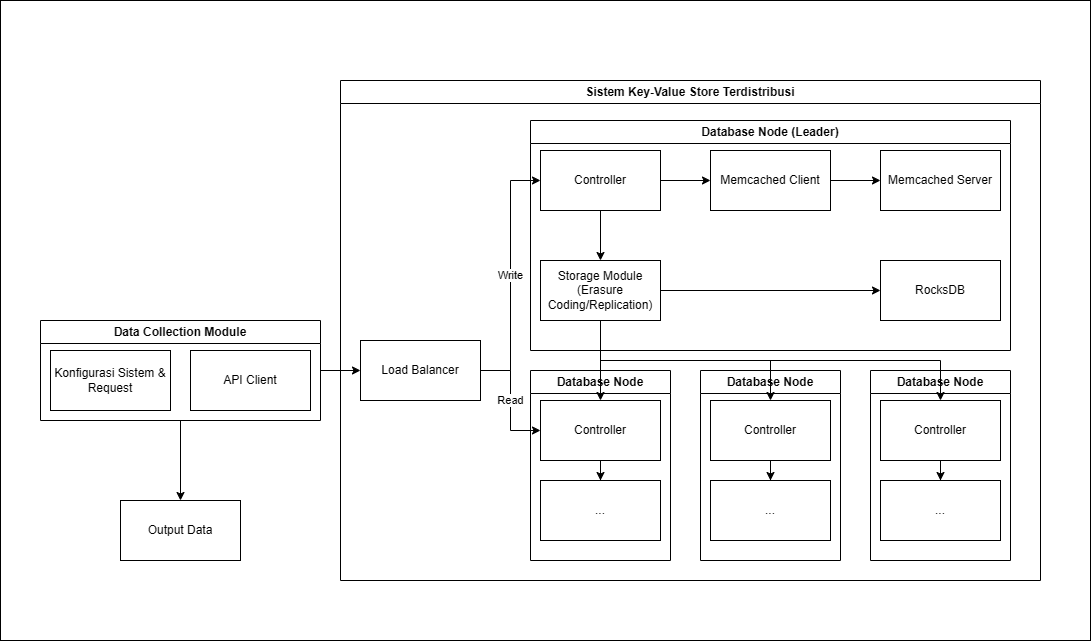
\includegraphics[width=0.95\textwidth]{resources/chapter-3/general-architecture.png}
    \caption{Gambaran Arsitektur Sistem Eksperimen}
    \label{fig:general-architecture}
\end{figure}

Arsitektur dari sistem mengasumsikan kebutuhan untuk konsistensi yang tinggi. Untuk mencapai konsistensi tersebut, operasi \textit{write} dilakukan secara \textit{synchronous} dengan distribusi replikasi dan \textit{erasure coding} dianggap selesai ketika nilai ketahanan yang diinginkan sudah tercapai.

Karena sistem bersifat terdistribusi, maka diperlukan sebuah algoritma konsensus untuk mengelola konsistensi antar \textit{Node}. Algoritma konsensus yang digunakan algoritma konsensus \textit{paxos} yang disesuaikan dengan kebutuhan. Salah satu penyesuaian yang dilakukan adalah mengadopsi pola \textit{leader-follower} untuk memudahkan sinkronisasi data dan mempercepat transaksi. Dengan adanya leader, fase 1 dari algoritma \textit{paxos} dapat dihilangkan dengan membuat proposal dari leader selalu memiliki nilai paling tinggi. Detail implementasi \textit{paxos} akan dijelaskan di bagian \ref{subsection:detail-komponen}. Diagram gambaran arsitektur sistem dapat dilihat pada gambar \ref{fig:general-architecture}.

Operasi \textit{write} akan secara ekslusif disalurkan pada \textit{leader}. Kemudian untuk ketahanan, data akan didistribusikan pada \textit{follower} sesuai dengan konfigurasi \textit{node}. Sementara itu, operasi \textit{read} dapat dilakukan pada \textit{Node} manapun. Pada sistem \textit{erasure coding}, jika pada \textit{node} tersebut tidak terdapat nilai data yang dicari, maka \textit{Node} akan melakukan \textit{request} ke semua node lainnya untuk melakukan rekonstruksi data.


\subsection{Alur Transaksi}
\label{subsection:system-flow}

Alur untuk transaksi \textit{read} dapat dilihat pada gambar \ref{fig:flow-read-mermaidjs} dengan \textit{request} masuk ke \textit{load balancer} kemudian disalurkan ke \textit{database node} yang tersedia. \textit{Database node} akan melakukan operasi \textit{read} pada \textit{key-value store} dan mengembalikan hasil operasi ke \textit{load balancer} untuk dikirimkan ke \textit{client} jika tersedia. Jika tidak, maka \textit{database node} akan melakukan rekonstruksi data dari \textit{erasure-coded persistent data} yang tersebar pada \textit{node-node} lainnya. Pada replikasi, data akan diambil dari \textit{node} lain yang memiliki data yang sama.

\begin{figure}[!ht]
    \centering
    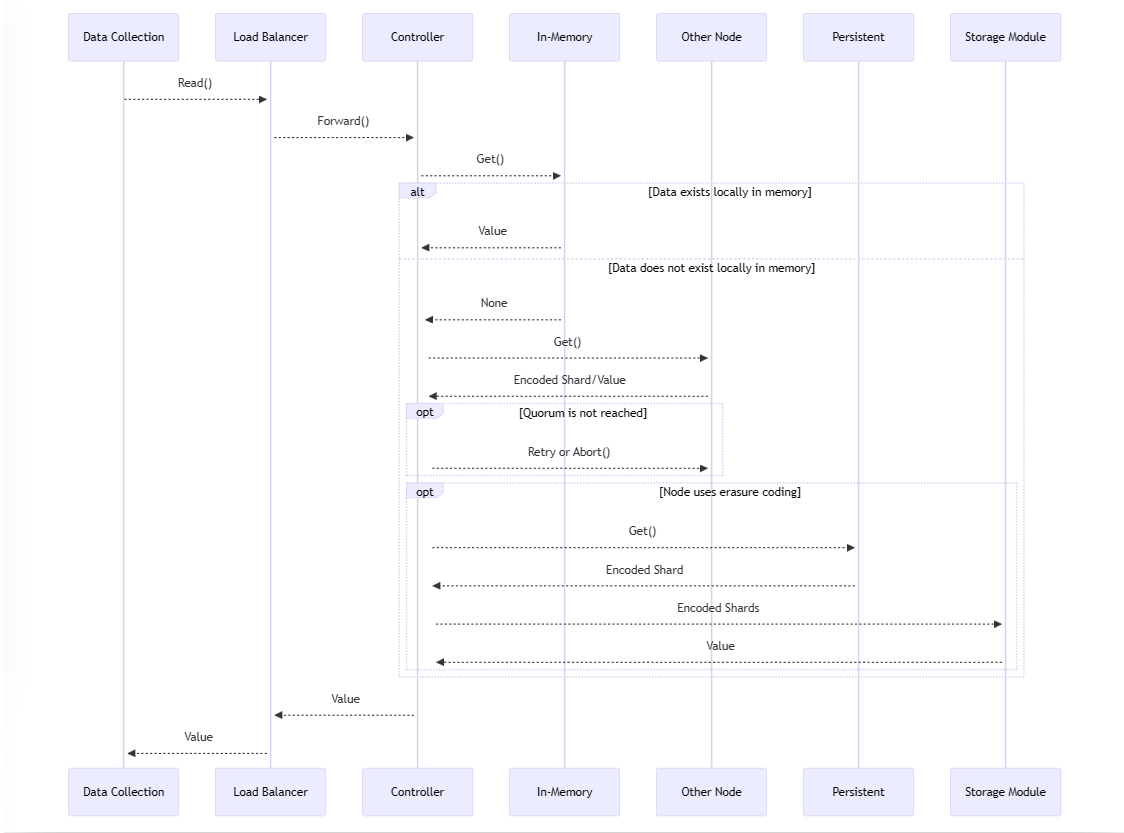
\includegraphics[width=0.95\textwidth]{resources/chapter-3/flow-read-mermaidjs.png}
    \caption{Flow operasi \textit{read} dalam rancangan implementasi}
    \label{fig:flow-read-mermaidjs}
\end{figure}

Alur untuk transaksi \textit{read} dapat dilihat pada gambar \ref{fig:flow-write-mermaidjs} dengan \textit{request} masuk ke \textit{load balancer} kemudian disalurkan ke \textit{database node} yang merupakan leader. Leader kemudian akan melakukan operasi \textit{erasure coding} lalu menyebarkan \textit{shard} ke \textit{follower} yang tersedia. Setelah semua \textit{follower} menerima \textit{shard}, maka operasi \textit{write} dianggap selesai. Operasi \textit{write} pada replikasi juga akan menunggu semua \textit{follower} menerima data sebelum dianggap selesai. 

\begin{figure}[!ht]
    \centering
    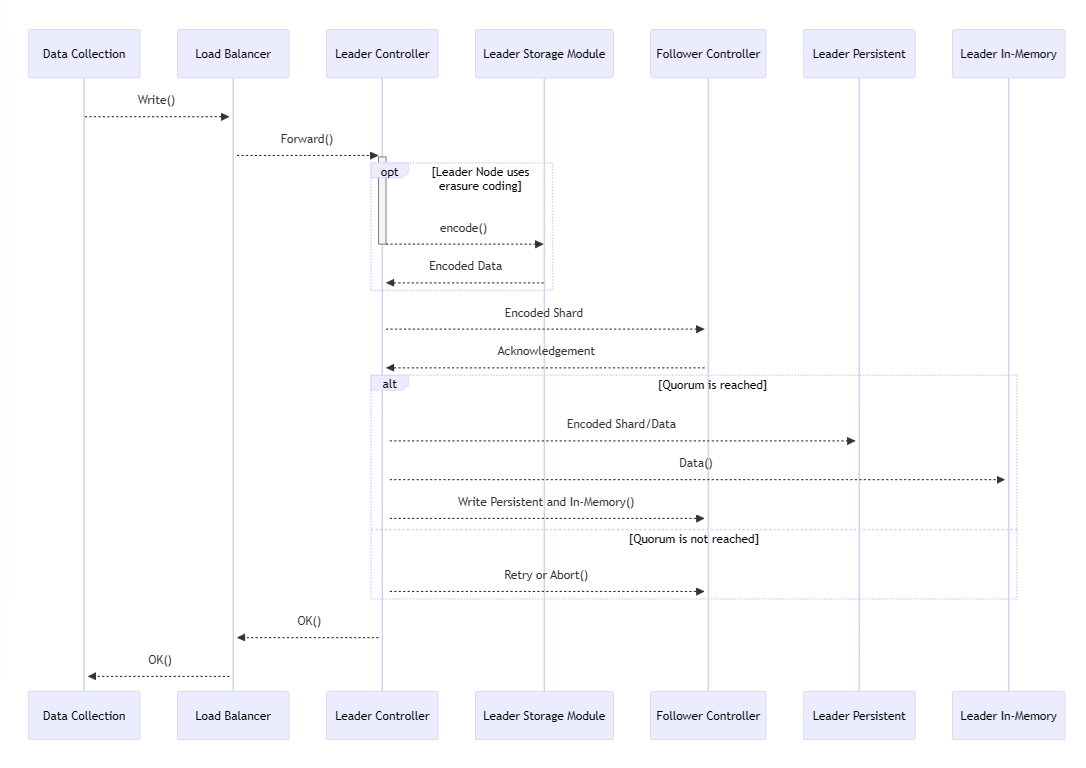
\includegraphics[width=0.95\textwidth]{resources/chapter-3/flow-write-mermaidjs.png}
    \caption{Flow operasi \textit{write} dalam rancangan implementasi}
    \label{fig:flow-write-mermaidjs}
\end{figure}


\subsection{Rancangan Detail Komponen}
\label{subsection:detail-komponen}

Berdasarkan rancangan struktural yang sudah dijelaskan pada bagian \ref{subsection:rancangan-struktural}, sistem akan diimplementasikan sebagai kumpulan komponen. Masing-masing komponen tersebut memiliki peran dan tanggung jawab yang berbeda dalam sistem eksperimen. Pada bagian ini, akan dijelaskan lebih lanjut mengenai rancangan detail dari masing-masing komponen tersebut.

\subsection{Rancangan Detail Node}
\label{subsection:detail-node}

Seperti yang sudah dijelaskan pada bagian \ref{sec:rancangan-struktural}, \textit{Node} merupakan satuan fungsional utama yang berperan sebagai entitas dalam sistem \textit{database} terdistribusi yang dikembangkan.

Struktur \textit{Node} terdiri dari:

\begin{enumerate}
    \item Subsistem penyimpanan: Subsistem ini bertanggung jawab untuk fungsionalitas \textit{key-value store} dalam sebuah \textit{Node}. Detail dari subsistem penyimpanan akan dijelaskan pada bagian \ref{subsection:detail-subsistem-penyimpanan}.
    \item Subsistem kontrol: Subsistem ini bertanggung jawab mengelola transaksi dan konsistensi antar-\textit{Node}. Detail dari subsistem kontrol akan dijelaskan pada bagian \ref{subsection:detail-subsistem-kontrol}.
    \item Komponen HTTP \textit{server}: Komponen ini berperan sebagai antarmuka komunikasi antara \textit{client} dan \textit{Node}. Detail dari komponen HTTP \textit{server} akan dijelaskan pada bagian \ref{subsection:detail-komponen-HTTP-server}.
    \item Komponen komunikasi antar-\textit{Node}: Komponen ini berfungsi untuk mengelola komunikasi antar-\textit{Node} dalam sistem terdistribusi. Detail dari komponen komunikasi antar-\textit{Node} akan dijelaskan pada bagian \ref{subsection:detail-subsistem-komunikasi-antar-node}.
\end{enumerate}

Ilustrasi struktur \textit{Node} dapat dilihat pada gambar \ref{fig:node-structure}.

% _TODO: Change image
\begin{figure}[ht]
    \centering
    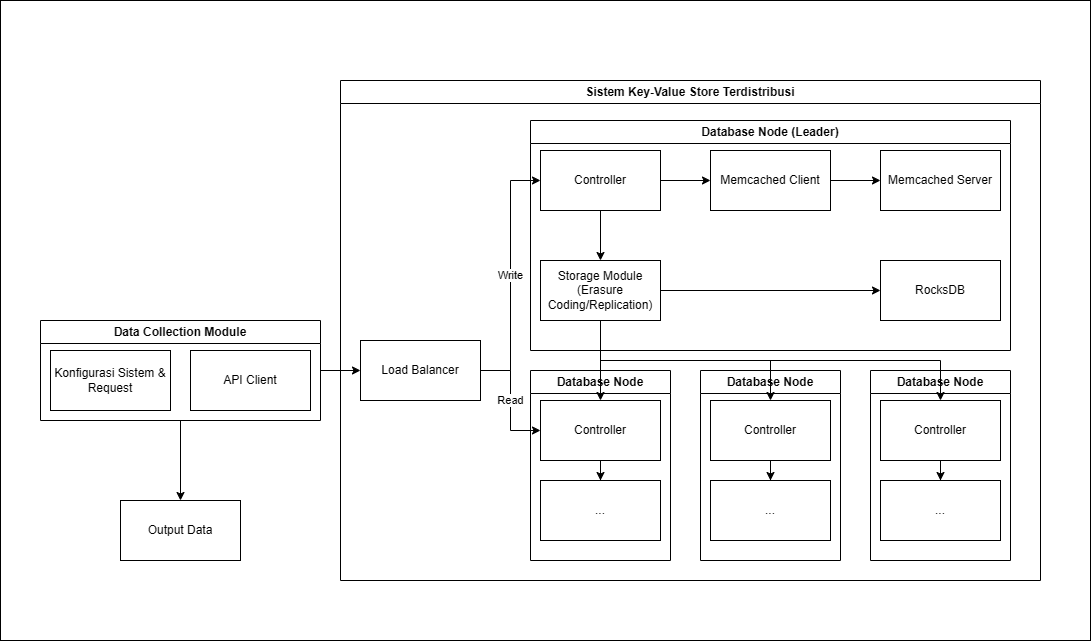
\includegraphics[width=0.95\textwidth]{resources/chapter-3/general-architecture.png}
    \caption{Struktur Node}
    \label{fig:node-structure}
\end{figure}
\subsubsection{Rancangan Detail Subsistem Penyimpanan}
\label{subsubsection:detail-subsistem-penyimpanan}

Subsistem penyimpanan adalah subsistem yang bertanggung jawab untuk fungsionalitas \textit{key-value store} dalam sebuah \textit{Node}. Subsistem ini akan terdiri atas komponen \textit{in-memory store}, \textit{persistent store}, \textit{transaction log}. Subsistem ini juga mengkonfigurasi \textit{Node} untuk menggunakan replikasi atau \textit{erasure coding}.

Mengikuti solusi yang sudah dipilih pada bagian \ref{sec:alternatif-solusi}, subsistem penyimpanan bersifat modular dengan Memcached sebagai \textit{in-memory key-value store} dan RocksDB sebagai \textit{persistent storage}. Memcached memiliki struktur \textit{server} dan \textit{client} sehingga subsistem ini berisi \textit{client} Memcached untuk berkomunikasi dengan \textit{server}. Pada rancangannya, dalam satu perangkat akan dijalankan satu \textit{server} Memcached untuk tiap \textit{Node} yang ada. Sementara itu, RocksDB dapat dijalankan pada tiap node tanpa memerlukan \textit{server}.

Ilustrasi struktur subsistem penyimpanan dapat dilihat pada gambar \ref{fig:storage-subsystem-structure}.

% _TODO: Change image
\begin{figure}[ht]
    \centering
    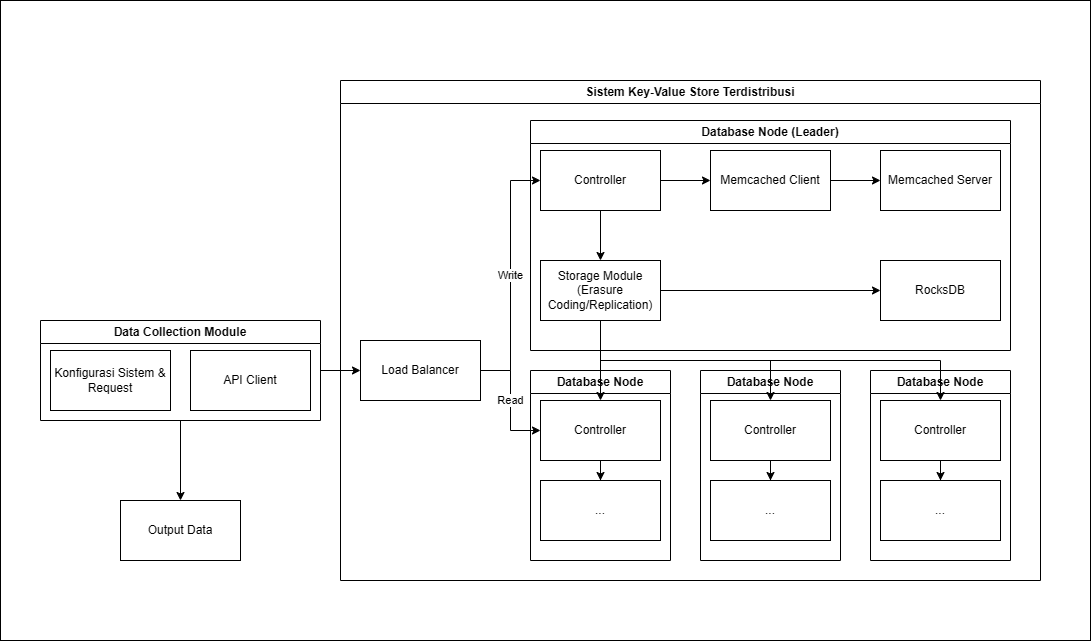
\includegraphics[width=0.95\textwidth]{resources/chapter-3/general-architecture.png}
    \caption{Struktur Subsistem Penyimpanan}
    \label{fig:storage-subsystem-structure}
\end{figure}

\subsubsection{Rancangan Detail Subsistem Kontrol}
\label{subsubsection:detail-subsistem-kontrol}
\subsubsection{Rancangan Detail Komponen HTTP Server}
\label{subsubsection:detail-komponen-HTTP-server}

Komponen HTTP \textit{server} berfungsi sebagai antarmuka komunikasi antara \textit{client} dan \textit{Node}. Komponen ini bertanggung jawab untuk menerima dan memproses permintaan dari \textit{client}, serta mengirimkan respons yang sesuai.

Ilustrasi struktur komponen HTTP \textit{server} dapat dilihat pada gambar \ref{fig:http-server-structure}.

% _TODO: Change image
\begin{figure}[ht]
    \centering
    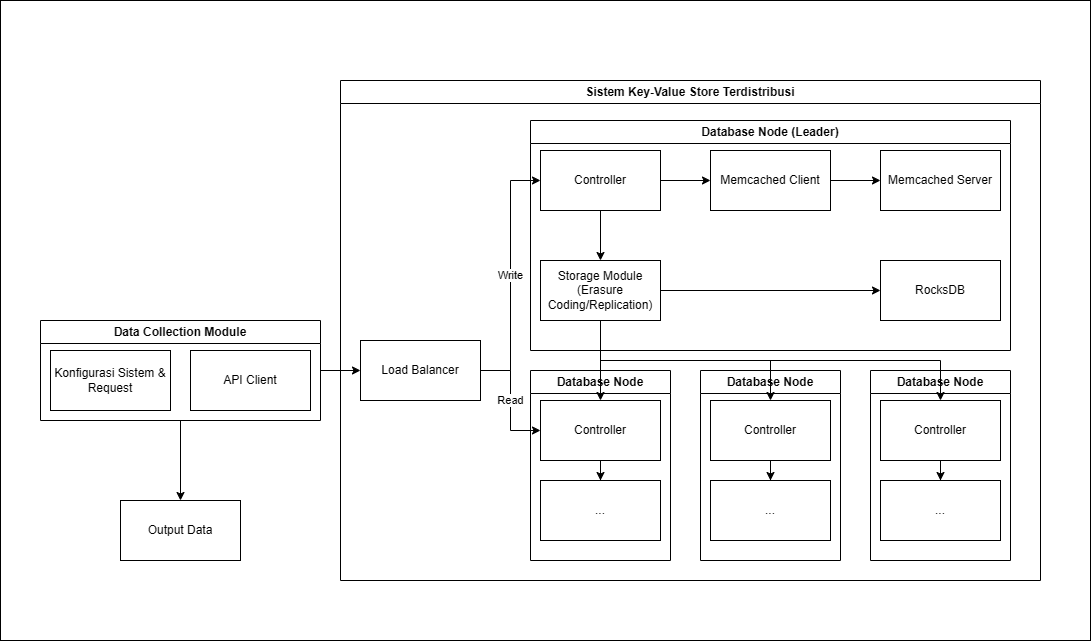
\includegraphics[width=0.95\textwidth]{resources/chapter-3/general-architecture.png}
    \caption{Struktur Komponen HTTP Server}
    \label{fig:http-server-structure}
\end{figure}

\subsubsection{Rancangan Detail Komponen Komunikasi Antar-Node}
\label{subsubsection:detail-subsistem-komunikasi-antar-node}

Komponen komunikasi antar-\textit{Node} bertanggung jawab untuk mengelola komunikasi antar-\textit{Node} dalam sistem terdistribusi. Komponen ini akan menggunakan protokol komunikasi yang sesuai untuk memastikan bahwa data dapat dikirim dan diterima.

Ilustrasi struktur komponen komunikasi antar-\textit{Node} dapat dilihat pada gambar \ref{fig:node-communication-structure}.

% _TODO: Change image
\begin{figure}[ht]
    \centering
    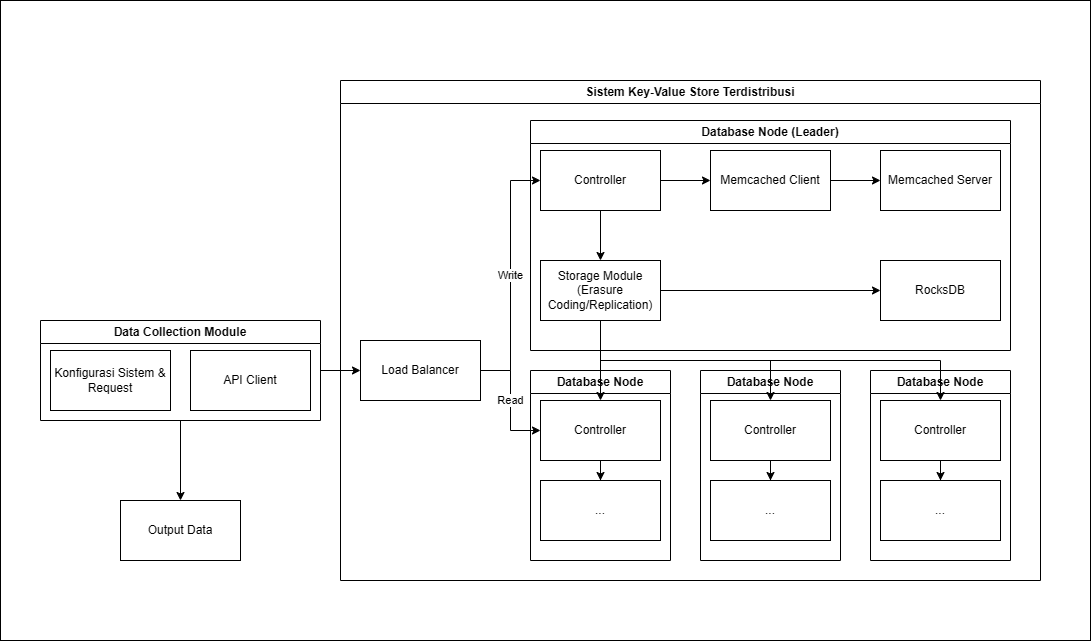
\includegraphics[width=0.95\textwidth]{resources/chapter-3/general-architecture.png}
    \caption{Struktur Komponen Komunikasi Antar-Node}
    \label{fig:node-communication-structure}
\end{figure}
\subsection{Rancangan Detail Data Collector}
\label{subsection:detail-data-collector}

Data Collector adalah komponen yang bertanggung jawab untuk mengumpulkan data dari sistem dan menyimpannya dalam format yang sesuai untuk analisis lebih lanjut. Komponen ini akan mengumpulkan data dari berbagai sumber, termasuk log sistem, metrik kinerja, dan informasi lainnya yang relevan.
Data Collector juga akan menyediakan antarmuka untuk mengakses data yang telah dikumpulkan, sehingga memudahkan pengguna untuk melakukan analisis dan visualisasi data.

Struktur \textit{Data Collector} terdiri dari:

\begin{enumerate}
    \item Komponen testing: Komponen ini bertanggung jawab untuk melakukan \textit{request} dan transaksi pada sistem.
    \item Komponen \textit{logging} dan \textit{tracing}: Komponen ini mengelola pencatatan dan pelacakan operasi yang dilakukan oleh sistem secara keseluruhan.
    \item Komponen \textit{reporting}: Komponen ini bertanggung jawab untuk mengumpulkan dan menyajikan hasil eksperimen dalam bentuk laporan.
\end{enumerate}

Ilustrasi struktur Data Collector dapat dilihat pada gambar \ref{fig:data-collector-structure}.

% _TODO: Change image
\begin{figure}[ht]
    \centering
    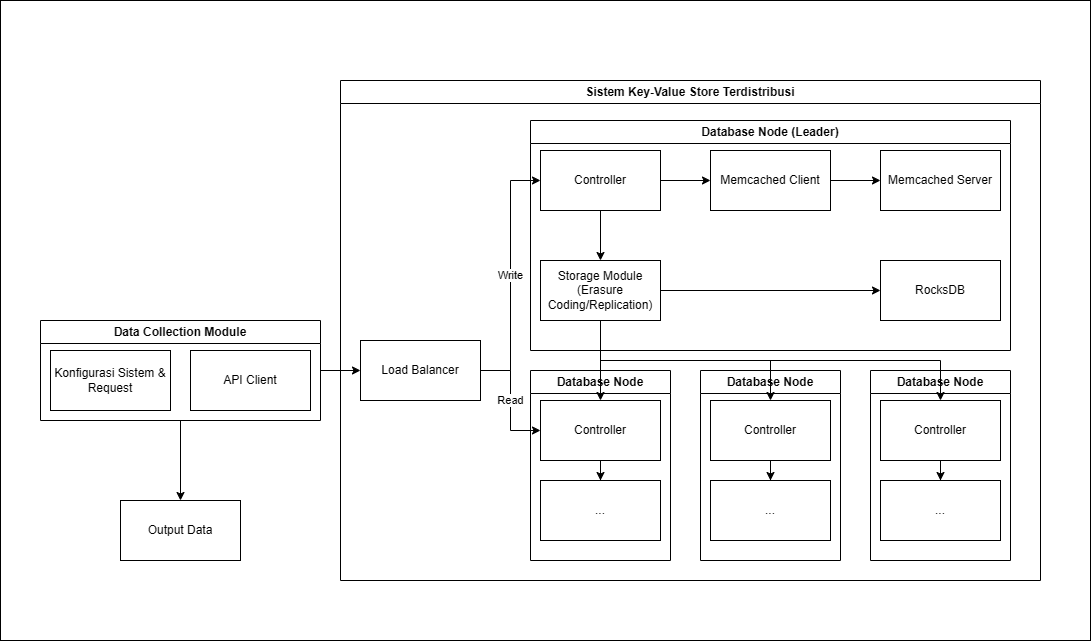
\includegraphics[width=0.95\textwidth]{resources/chapter-3/general-architecture.png}
    \caption{Struktur Data Collector}
    \label{fig:data-collector-structure}
\end{figure}
\subsubsection{Rancangan Detail Komponen Testing}
\label{subsubsection:detail-data-collector}

Komponen \textit{testing} bertanggung jawab untuk melakukan pengujian terhadap sistem yang telah dibangun. Pengujian ini dilakukan untuk memastikan bahwa sistem berfungsi sesuai dengan spesifikasi yang telah ditentukan. Komponen ini juga bertanggung jawab untuk menghasilkan data yang kemudian dimasukkan ke komponen \textit{reporting} untuk visualisasi dan analisis.

Ilustrasi struktur komponen \textit{testing} dapat dilihat pada gambar \ref{fig:testing-structure}.

% _TODO: Change image
\begin{figure}[ht]
    \centering
    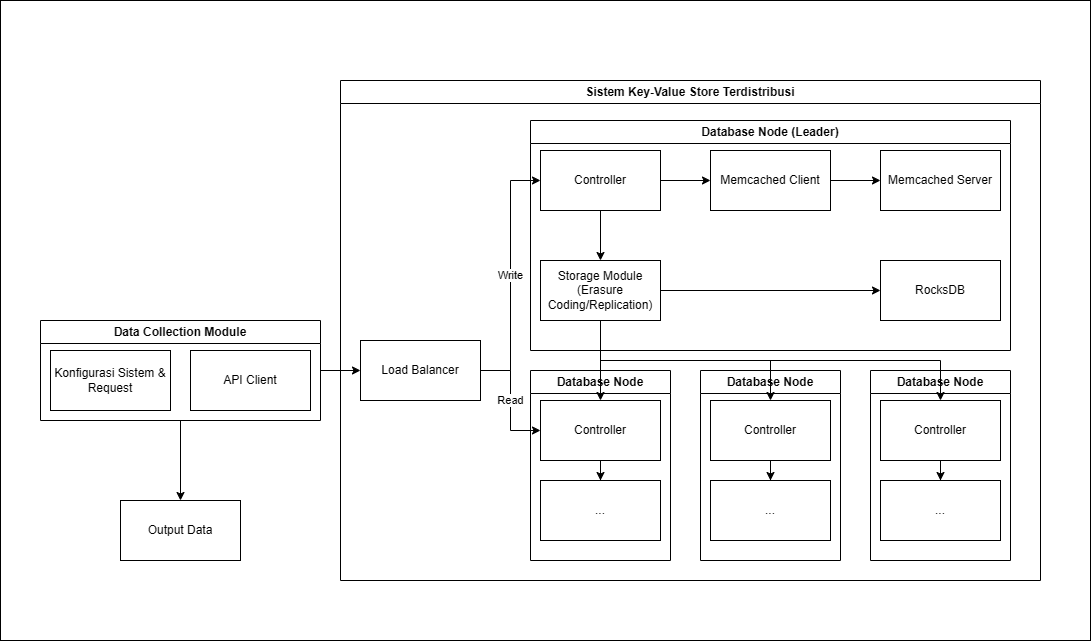
\includegraphics[width=0.95\textwidth]{resources/chapter-3/general-architecture.png}
    \caption{Struktur Komponen Testing}
    \label{fig:testing-structure}
\end{figure}
\subsubsection{Rancangan Detail Komponen Logging dan Tracing}
\label{subsubsection:detail-data-collector}

Komponen \textit{logging} dan \textit{tracing} bertanggung jawab untuk mencatat dan melacak aktivitas sistem. Komponen ini akan mengumpulkan data dari berbagai komponen lain dalam sistem, termasuk informasi tentang permintaan yang diterima, respons yang dikirim, dan status sistem secara keseluruhan. Data ini akan digunakan untuk analisis lebih lanjut dan pemecahan masalah.

Ilustrasi struktur komponen \textit{logging} dan \textit{tracing} dapat dilihat pada gambar \ref{fig:logging-tracing-structure}.

% _TODO: Change image
\begin{figure}[ht]
    \centering
    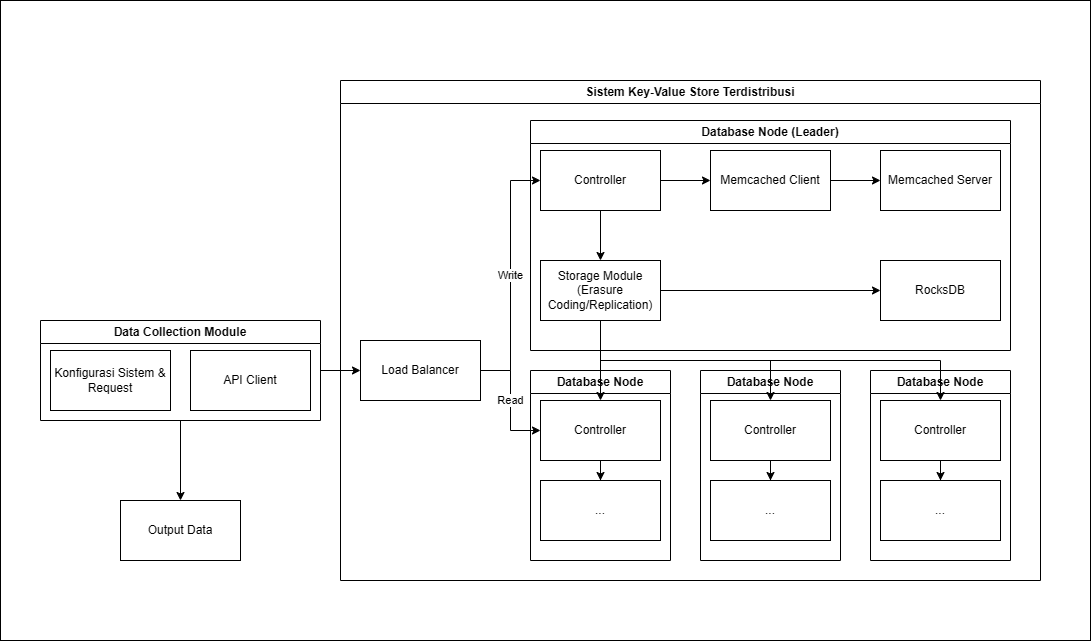
\includegraphics[width=0.95\textwidth]{resources/chapter-3/general-architecture.png}
    \caption{Struktur Komponen Logging dan Tracing}
    \label{fig:logging-tracing-structure}
\end{figure}
\subsubsection{Rancangan Detail Komponen Reporting}
\label{subsubsection:detail-reporting}

Komponen \textit{reporting} bertanggung jawab untuk menghasilkan laporan berdasarkan data yang telah dikumpulkan oleh komponen \textit{data collector}. Komponen ini akan memproses data dan menghasilkan visualisasi yang dapat digunakan untuk analisis lebih lanjut.

Ilustrasi struktur komponen \textit{reporting} dapat dilihat pada gambar \ref{fig:reporting-structure}.

% _TODO: Change image
\begin{figure}[ht]
    \centering
    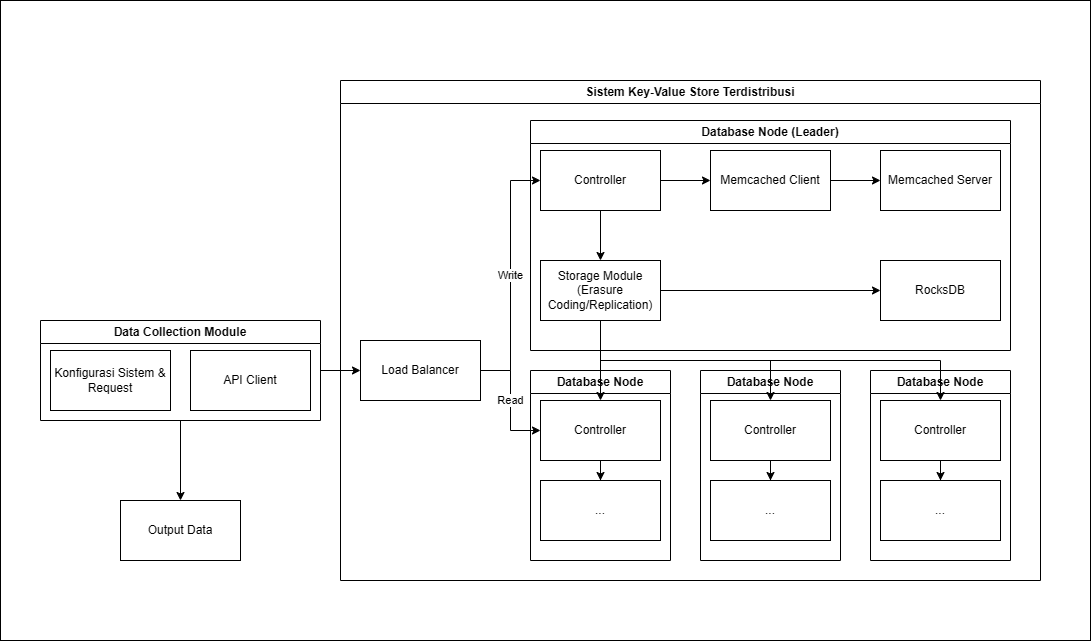
\includegraphics[width=0.95\textwidth]{resources/chapter-3/general-architecture.png}
    \caption{Struktur Komponen Reporting}
    \label{fig:reporting-structure}
\end{figure}

